% 第9章第1节：线性空间与子空间（向量空间；子空间及其包含、交、和、直和与商空间）。

\section{线性空间与子空间}
\label{sec:ls-vector-spaces}
\label{sec:linear-algebra-vector-spaces-coordinates}

第~\ref{chap:linear-operations}章的数组和本章开头的仿射函数都能相加和缩放。用一组方向记录这些对象之前，要先说清线性组合在什么范围内进行。本节先给出线性空间的定义，再讨论空间内部对线性组合封闭的部分，即子空间，以及子空间之间的比较、合并和商空间。

\subsection{线性空间的定义与示例}
\label{sec:ls-space-axioms}

第~\ref{sec:ls-vector-operation-rules}节验证过，同形数组的加法与数乘满足八条运算规则。其他对象也满足同样的规则：平面上的位移可以首尾相接，有限信号可以按幅度放大，多项式可以逐点相加。后面关于分解、方程的解和维数的结论只用到这八条规则，与对象具体是数组、位移、信号还是多项式无关。因此，把带有这样的加法与数乘的集合统称为线性空间，其中的元素统称为向量。从此，“向量”指可以作线性组合的对象，不再要求它是一列数。

\begin{definition}[实线性空间]
\label{def:ls-real-vector-space}
设$V$是一个集合，给定加法（任意$\bm u,\bm v\in V$对应$\bm u+\bm v\in V$）与实数数乘（任意$a\in\mathbb R$、$\bm u\in V$对应$a\bm u\in V$）。若对任意$\bm u,\bm v,\bm w\in V$和$a,b\in\mathbb R$，下面八条规则成立，就称$V$为\term{向量空间}（也称线性空间，vector space）：
\begin{enumerate}
 \item 加法交换律：$\bm u+\bm v=\bm v+\bm u$。
 \item 加法结合律：$(\bm u+\bm v)+\bm w=\bm u+(\bm v+\bm w)$。
 \item 零元：存在$\bm0\in V$，使$\bm u+\bm0=\bm u$对每个$\bm u$成立。
 \item 加法逆元：每个$\bm u$都有$-\bm u\in V$，使$\bm u+(-\bm u)=\bm0$。
 \item 数乘结合律：$a(b\bm u)=(ab)\bm u$。
 \item 数乘对数的分配律：$(a+b)\bm u=a\bm u+b\bm u$。
 \item 数乘对向量的分配律：$a(\bm u+\bm v)=a\bm u+a\bm v$。
 \item 单位数乘：$1\bm u=\bm u$。
\end{enumerate}
\end{definition}
定义包含两层要求。第一层是\emph{封闭}：加法和数乘的结果必须留在$V$中，否则运算无法在$V$内进行。第二层是\emph{规则}：前四条说加法像数的加法一样可以交换、结合，有零元和相反元；后四条说数乘与加法按熟悉的方式配合。

有了这些规则，有限次线性运算无论怎样加括号、怎样展开，结果都相同。所以对任意$\bm v_1,\ldots,\bm v_k\in V$与实数$a_1,\ldots,a_k$，加权和$\sum_{j=1}^ka_j\bm v_j$有确定的意义。它仍称为这组向量的线性组合，与第~\ref{sec:ls-vector-operations}节对数组的定义一致。

标量也可以取复数。复线性空间满足同样的八条规则，只是数乘允许任意复数。允许哪些标量会改变线性结构。$\mathbb C$作为复线性空间时，每个元素都是$1$的复数倍；只允许实数数乘时，表示$a+b\mathrm i$需要$1$与$\mathrm i$两个方向。复数域上的基与线性映射按同样的方式定义，内积则要处理共轭。本章其余推导在实数域中进行。

常见的具体空间都满足定义。$\mathbb R^d$与全体$m\times d$实矩阵在逐项运算下是线性空间，第~\ref{sec:ls-vector-operation-rules}节已逐条验证。次数不超过$k$的实多项式组成的集合
\[
 P_k=\{a_0+a_1t+\cdots+a_kt^k:a_0,\ldots,a_k\in\mathbb R\}
\]
在逐点相加与数乘下也是线性空间：两个这样的多项式相加或乘以实数，次数仍不超过$k$；八条规则则逐点继承实数运算的规则。本章开头的仿射函数全体正是$P_1$。

并非每个由向量组成的集合都是线性空间。下面两个$\mathbb R^d$的子集沿用$\mathbb R^d$的运算，分别破坏了加法封闭与数乘封闭。
\begin{example}[反例：仿射约束集与非负向量集]
\label{ex:ls-non-vector-space-sets}
给定：$\mathbb R^d$的两个子集
\[
 \begin{gathered}
S_1=\{\bm x\in\mathbb R^d:x_1=1\}\\
S_2=\{\bm x\in\mathbb R^d:x_j\geq0,\ j=1,\ldots,d\},
 \end{gathered}
\]
运算沿用$\mathbb R^d$的逐项加法与数乘。

验证：任取$\bm x,\bm y\in S_1$，和的第一坐标为$x_1+y_1=2\neq1$，所以$\bm x+\bm y\notin S_1$；零向量的第一坐标为$0$，所以$S_1$也不含零向量。两个非负向量之和仍非负，所以$S_2$对加法封闭；但$\bm e_1\in S_2$，而$(-1)\bm e_1$的第一坐标为$-1$，不属于$S_2$。

结论：$S_1$对加法不封闭，$S_2$对数乘不封闭，二者都不是线性空间。
\end{example}
可见，判断一个集合是不是线性空间，要逐项检查运算是否封闭、规则是否成立，不能只看集合的形状。

\subsection{子空间、和与直和}
\label{sec:ls-subspaces}
\label{sec:linear-algebra-relations}
\label{sec:linear-algebra-subspace-relations}
\label{sec:ls-subspace-definition}

线性空间中常有一部分元素自己构成线性空间，例如平面中过原点的直线、齐次方程组的全部解。后面要处理的许多对象都是这样的部分：一组方向能到达的对象、一个映射消去的输入、方程的解，一般都只占空间的一部分。下面先给出判定条件，再比较和合并这些部分。

\paragraph{子空间的判定}
设$U$是$V$的非空子集。若$U$对线性组合封闭，即对任意$\bm u,\bm v\in U$和$a,b\in\mathbb R$都有$a\bm u+b\bm v\in U$，就称$U$为$V$的\term{线性子空间}（linear subspace），简称子空间。

这一条件已足以保证$U$在$V$的运算下构成线性空间。取$a=b=1$得加法封闭，取$b=0$得数乘封闭；取$a=b=0$得$\bm0\in U$，取$a=-1$、$b=0$得$-\bm u\in U$。其余规则对$V$的全部元素成立，自然也对$U$的元素成立。所以判断子空间只需检查这一条封闭条件，不必逐条核对八条规则。

每个空间都有两个平凡子空间：只含零向量的$\{\bm0\}$和$V$本身。下面用判定条件检查三个常见集合。
\begin{example}[过原点的直线、平移的直线与齐次解集]
\label{ex:ls-subspace-checks}
给定：平面中的非零向量$\bm u$，不在直线$\{c\bm u:c\in\mathbb R\}$上的点$\bm p$，以及矩阵$\bm A\in\mathbb R^{m\times d}$。考察
\[
 \begin{gathered}
 L_0=\{c\bm u:c\in\mathbb R\},
 \qquad
 L_1=\{\bm p+c\bm u:c\in\mathbb R\},\\
 N=\{\bm x\in\mathbb R^d:\bm A\bm x=\bm0\}.
 \end{gathered}
\]

验证：在$L_0$中任取$c_1\bm u$与$c_2\bm u$，有$a(c_1\bm u)+b(c_2\bm u)=(ac_1+bc_2)\bm u\in L_0$。在$N$中任取两个解$\bm x,\bm y$，由式~\eqref{eq:prelim-matrix-linearity}，
\[
 \bm A(a\bm x+b\bm y)=a\bm A\bm x+b\bm A\bm y=\bm0,
\]
所以$a\bm x+b\bm y\in N$。$L_1$不含零向量：若$\bm p+c\bm u=\bm0$，则$\bm p=-c\bm u$落在$L_0$上，与$\bm p$的取法矛盾。

结论：过原点的直线$L_0$与齐次线性方程组的解集合$N$都是子空间；不过原点的直线$L_1$不含零向量，不是子空间。
\end{example}
$L_1$由子空间$L_0$沿$\bm p$平移得到。示例~\ref{ex:ls-non-vector-space-sets}中的约束集$S_1=\{\bm x:x_1=1\}$也是如此：它由齐次解集$\{\bm x:x_1=0\}$沿$\bm e_1$平移得到，是一个仿射集合，同样不是子空间。

同一个空间$V$中的几个子空间可以从四个方面比较：一个是否含于另一个，二者有哪些公共向量，合起来能到达哪里，合并后的分解是否唯一。这四个方面分别由包含、交、和与直和描述。它们只涉及线性组合，不涉及长度或夹角。

\paragraph{包含}
\phantomsection
\label{sec:ls-subspace-inclusion}
若子空间$U$的每个元素都属于子空间$W$，就记$U\subseteq W$。这时$U$在$W$中对线性组合封闭，因而也是$W$的子空间。包含只比较两个集合的范围；两个子空间的“大小”要等下一节定义了维数才能比较。

\paragraph{交}
\phantomsection
\label{sec:ls-intersection}
两个子空间$U,W\subseteq V$的交$U\cap W$由同时属于二者的元素组成。它仍是子空间：若$\bm x,\bm y\in U\cap W$，则二者同在$U$中，也同在$W$中，所以$a\bm x+b\bm y$同属两边。任何同时含于$U$与$W$的子空间，其元素都属于交，所以交是同时含于二者的最大子空间。

在平面中，两条重合的过原点直线的交是整条直线，两条不同的过原点直线的交只有零向量。交为零只说明两个子空间没有公共的非零向量，不说明二者合起来能到达整个空间。例如$\mathbb R^3$中两条不同的过原点直线交为零，合起来只能到达一个平面。

当$U,W$分别由齐次线性方程组描述时，交就是同时满足两组方程的解集合。例如$U=\{\bm x:x_1=0\}$与$W=\{\bm x:x_2=0\}$的交是$\{\bm x:x_1=x_2=0\}$。求交因此化为解联立的齐次方程组，消元方法见第~\ref{chap:linear-equations-and-optimization}章。

\paragraph{和}
\phantomsection
\label{sec:ls-sum}
把两个子空间中的向量相加，能得到的全部向量组成和空间
\[
 U+W=\{\bm u+\bm w:\bm u\in U,\ \bm w\in W\}.
\]
它对线性组合封闭：
\[
 a(\bm u_1+\bm w_1)+b(\bm u_2+\bm w_2)=(a\bm u_1+b\bm u_2)+(a\bm w_1+b\bm w_2),
\]
右端两个括号分别属于$U$与$W$。任何同时包含$U$与$W$的子空间都必须含有每个$\bm u+\bm w$，所以$U+W$是同时包含二者的最小子空间。

同时包含$U$与$W$的最小集合是并集$U\cup W$，但并集一般对加法不封闭，不能代替和空间。
\begin{example}[反例：两条坐标轴的并]
\label{ex:ls-union-not-subspace}
给定：$\mathbb R^2$中的两个子空间$U=\{(s,0)^\top:s\in\mathbb R\}$与$W=\{(0,s)^\top:s\in\mathbb R\}$，即两条坐标轴。

验证：$\bm e_1\in U$、$\bm e_2\in W$，二者都属于$U\cup W$；但$\bm e_1+\bm e_2=(1,1)^\top$的两个坐标都不为零，既不在$U$中，也不在$W$中。

结论：$U\cup W$对加法不封闭，不是子空间；包含$U$与$W$的最小子空间是$U+W=\mathbb R^2$。
\end{example}
和空间就是在并集之外补入了$\bm u+\bm w$这类必需的线性组合。

\paragraph{直和与补空间}
\phantomsection
\label{sec:ls-direct-sum}
和空间中的向量都能写成$\bm u+\bm w$，但写法未必唯一。在平面上取两条不平行的过原点直线，每个向量都能拆成分别落在两条直线上的两部分，而且拆法唯一。唯一与否由两个子空间的交决定。
\begin{theorem}[和的分解唯一的条件]
\label{thm:ls-direct-sum-uniqueness}
设$U,W$是$V$的子空间。$U+W$中每个向量写成$\bm u+\bm w$（$\bm u\in U$，$\bm w\in W$）的方式都唯一，当且仅当
\[
 U\cap W=\{\bm0\}.
\]
\end{theorem}
\begin{proof}
充分性：若$\bm u_1+\bm w_1=\bm u_2+\bm w_2$，移项得$\bm u_1-\bm u_2=\bm w_2-\bm w_1$。左边在$U$中，右边在$W$中，所以这个向量属于$U\cap W$，只能是零。于是$\bm u_1=\bm u_2$，$\bm w_1=\bm w_2$。

必要性：若交中有非零向量$\bm z$，则$\bm z\in U$、$-\bm z\in W$，等式$\bm0=\bm0+\bm0=\bm z+(-\bm z)$给出零向量的两种不同分解，唯一性不成立。
\end{proof}

满足$U\cap W=\{\bm0\}$时，称和$U+W$为\term{直和}（direct sum），记为$U\oplus W$。唯一分解不要求两个子空间互相垂直：平面中任意两条不平行的过原点直线都构成直和。

若还有$U+W=V$，就写$V=U\oplus W$，并称$W$为$U$在$V$中的\term{补空间}（complement）。补空间一般不唯一：平面中一条过原点的直线，以任何不平行于它的过原点直线为补空间。

补空间总是存在，证明要用到下一节的基扩充（第~\ref{sec:ls-dimension}节）。

\subsection{商空间}
\phantomsection
\label{sec:ls-quotient-spaces}
\label{sec:linear-algebra-equivalence-relations}
和与直和把子空间合并起来。有时需要反过来，有意忽略某个子空间内的差别。例如只关心仿射函数$f_{a,b}(t)=a+bt$在$t=0$处的值，即截距$a$时，$f_{a,b}$与$f_{a,b'}$没有区别；二者之差$(b-b')t$落在子空间$\{st:s\in\mathbb R\}$中。

非齐次约束$x_1=1$的解也有同样的结构。它的解集合$\{\bm e_1+\bm n:n_1=0\}$由一个特解加上齐次解子空间$\{\bm n:n_1=0\}$中的全部向量组成，任意两个解之差都落在这个子空间里。两个例子的共同点是：相差某个子空间中的向量，就视为相同。

把这一点写成关系。设$U$是$V$的子空间，规定$\bm x\sim\bm y$当且仅当$\bm x-\bm y\in U$。它是第~\ref{chap:sets-functions-and-proofs}章定义~\ref{def:prelim-equivalence-relation}意义下的等价关系：由$\bm x-\bm x=\bm0\in U$得自反性；由$\bm x-\bm y\in U$蕴含$\bm y-\bm x\in U$得对称性；由$(\bm x-\bm y)+(\bm y-\bm z)=\bm x-\bm z\in U$得传递性。

$\bm x$所在的等价类为
\[
 \bm x+U=\{\bm x+\bm n:\bm n\in U\},
\]
即子空间$U$沿$\bm x$平移所得的集合。两个类相等，不要求代表元相等，只要求代表元之差落在$U$中。全部等价类把$V$分成互不重叠的块。图~\ref{fig:ls-quotient-equivalence-classes}在平面上画出这种划分：$U$是$x$轴，每条平行于$x$轴的直线是一个等价类。
\begin{figure}[htbp]
  \centering
  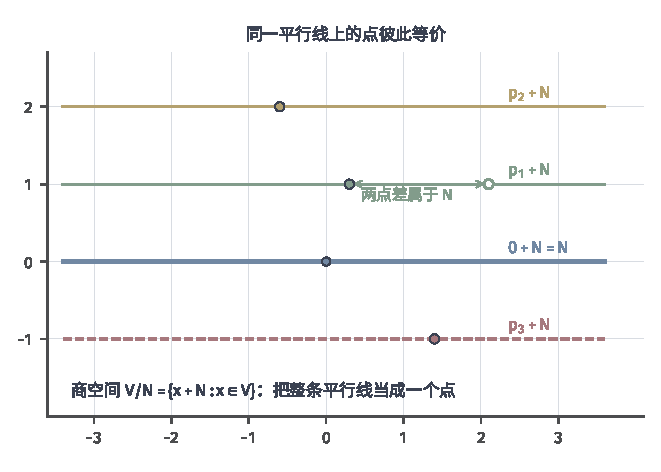
\includegraphics[width=112mm]{figures/00-shared/mathematical-preliminaries-upper/02-linear-spaces/matplotlib/ls-quotient-equivalence-classes/ls-quotient-equivalence-classes.pdf}
  \caption{商空间的等价类。$V=\mathbb R^2$，子空间$U$为$x$轴（蓝线$0+U$）；每条平行直线$p+U=\{(x,p_y)\}$是一个等价类，图中画出$y=1$（绿）、$y=2$（黄）、$y=-1$（红虚线）。绿线上实点$(0.3,1)$与空心点$(2.1,1)$之差$(1.8,0)\in U$，故属同一类；商空间$V/U$把每条平行线当成一个点。}
  \label{fig:ls-quotient-equivalence-classes}
\end{figure}

要让这些类像向量一样相加和缩放，自然的做法是对代表元作运算。
\begin{definition}[商空间]
\label{def:linear-algebra-quotient-space}
设$U$是线性空间$V$的子空间。全部等价类$\bm x+U$组成的集合记为$V/U$，规定
\[
 \begin{gathered}
(\bm x+U)+(\bm y+U)=(\bm x+\bm y)+U\\
a(\bm x+U)=a\bm x+U,
 \end{gathered}
\]
称$V/U$为$V$对$U$的\term{商空间}（quotient space）。
\end{definition}
借代表元定义运算，必须先检查结果与代表元的选取无关。把代表元换成$\bm x'=\bm x+\bm n_1$、$\bm y'=\bm y+\bm n_2$（$\bm n_1,\bm n_2\in U$）时，$\bm x'+\bm y'$与$\bm x+\bm y$只相差$\bm n_1+\bm n_2$，$a\bm x'$与$a\bm x$只相差$a\bm n_1$。二者都属于$U$，所以得到的类不变。

零类是$U$本身，$\bm x+U$的相反类是$-\bm x+U$，其余规则由$V$的运算规则逐条继承，所以$V/U$是线性空间。在图~\ref{fig:ls-quotient-equivalence-classes}中，两条水平线相加就是高度相加：商空间只记录高度，忽略了沿$x$轴的位置。

截距的例子可以照此计算。商空间恰好只保留截距。
\begin{example}[只保留截距的商空间]
\label{ex:ls-quotient-intercept}
给定：$V=P_1=\{a+bt:a,b\in\mathbb R\}$与子空间$U=\{st:s\in\mathbb R\}$。

计算：$f_{a,b}=a+bt$所在的类是
\[
 f_{a,b}+U=\{a+(b+s)t:s\in\mathbb R\}=\{a+rt:r\in\mathbb R\},
\]
它只依赖$a$。两个类$f_{a,b}+U$与$f_{a',b'}+U$相等，当且仅当$f_{a,b}-f_{a',b'}=(a-a')+(b-b')t\in U$，即$a=a'$。按商空间的运算，
\[
 \begin{gathered}
(f_{a,b}+U)+(f_{a',b'}+U)=f_{a+a',\,b+b'}+U\\
c(f_{a,b}+U)=f_{ca,\,cb}+U,
 \end{gathered}
\]
即截距分别相加、缩放。

结论：规则$f_{a,b}+U\mapsto a$是从$P_1/U$到$\mathbb R$的双射，并保持加法与数乘。商空间$P_1/U$只记录截距，忽略了斜率。
\end{example}
商空间的维数在第~\ref{sec:ls-dimension}节计算；它与线性映射的联系见第~\ref{sec:ls-kernel-image}节。
